\documentclass[12pt]{article}
\usepackage[utf8]{inputenc}
\usepackage[margin=1in]{geometry}
\usepackage{graphicx}
\usepackage{caption}
\usepackage{subcaption}

\usepackage[parfill]{parskip}
\usepackage{placeins}
\usepackage{csvsimple}
\usepackage{amsmath}

\usepackage{tikz}
\usetikzlibrary{positioning}

\begin{document}
\title{Discovering Patterns in Geometric Datasets}
\author{Alex Katzfey \& Paul Hein}
\maketitle

\section{Introduction}
Our project focused on creating a geometric pattern finding algorithm to discover repeated patterns in geometric data. For the purpose of this project we define geometric data as any data that can be represented as a set of k-dimensional tuples, where the possible values that any position in a tuple can take are countably infinite. This defines that the set of all possible \textit{k-tuples} is countably infinite. The motivation for such an algorithm is to use discovered patterns as constraints in the process of generating new geometric data with patterns from previously observed data.  We began our search for a good pattern finding algorithm by reading and implementing well-known algorithms from current literature. The algorithm we chose to study and implement for geometric data is called SIATEC. This is an algorithm that was created to find all maximal translatable patterns in a k-dimensional geometric dataset, and then group these patterns in translational equivalence classes.
\\
\\To understand this algorithm, and the new algorithm we will present we must define the terms maximal translatable pattern (MTP) and translational equivalence class (TEC). First, let us consider a 2-dimensional geometric dataset. The dataset provided in the visualization below will serve as our example dataset for understanding the SIATEC algorithm.

\FloatBarrier
\begin{figure}[!htbp]
  \centering
  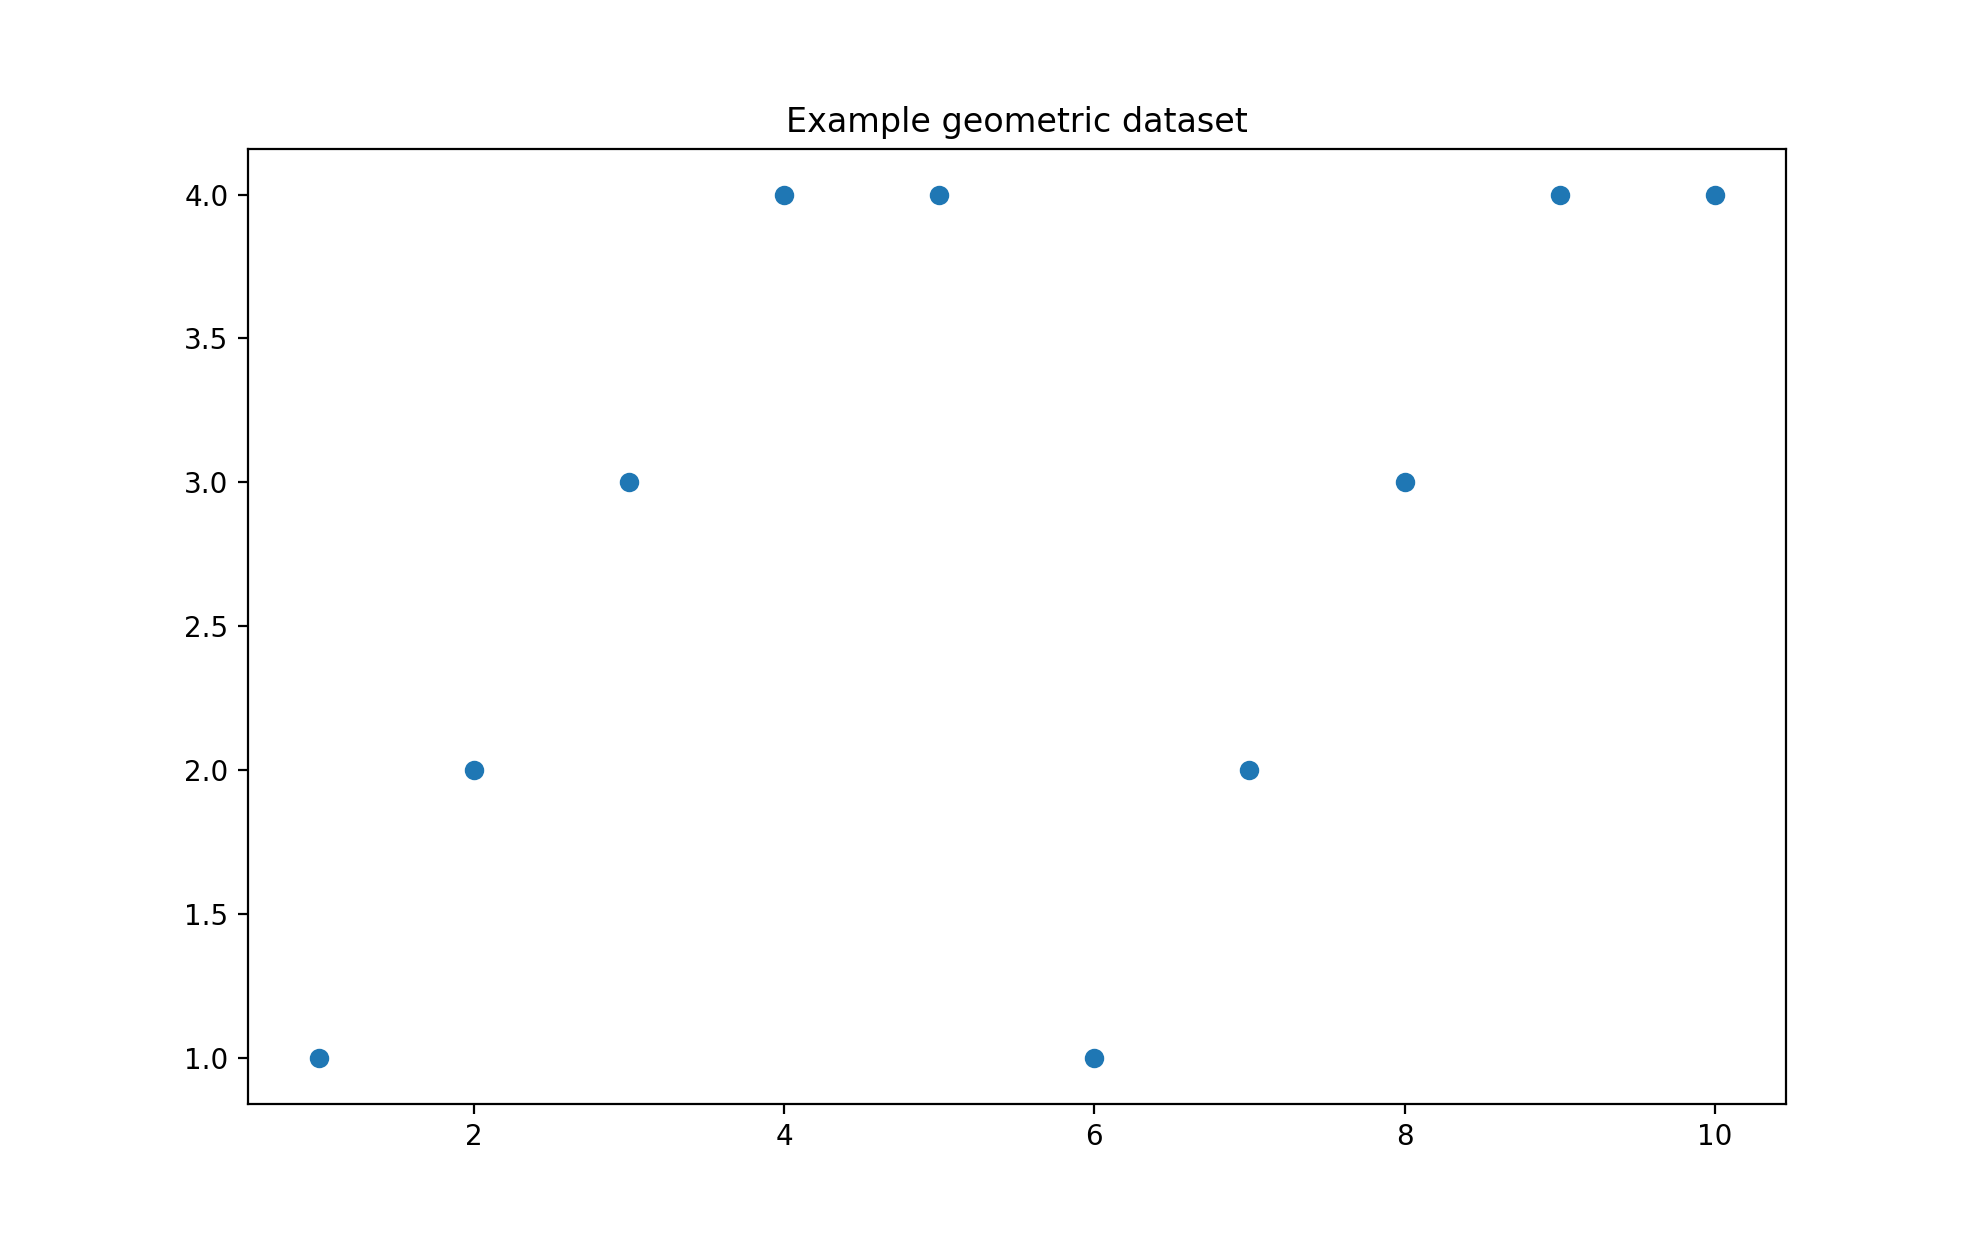
\includegraphics[width=.55\textwidth]{orig_data_example}
  \label{fig:figure1}
  \caption{Example 2-dimensional geometric dataset}
\end{figure}
\FloatBarrier

An MTP in this dataset is any maximal set of points in the dataset $D$ for which every point can be translated by the 2-dimensional vector $v$ to another position in $D$. The formal set theory definition of this object is included below:

$$MTP(v, D)  = \{ d ~|~ d \in D \land d + v \in D \}$$
\\
\\Computing the all MTPs of a dataset $D$ will return all instances of maximal patterns present in $D$. The final task is to remove duplicate patterns, and group similar patterns into TECs. Let us define duplicate patterns. An MTP $\{(1, 1); (2, 2); (3, 3)\}$ shifted by vector $(0, 2)$ is equivalent to the MTP $\{(1, 3); (2, 4); (3, 5)\}$ shifted by vector $(0, -2)$. Any pattern that seeks to find and group all similar patterns must account for the possibility of these duplicates occurring and remove them before outputting results. Now let us consider the definition of a TEC. Consider, again, the MTP $\{(1, 1); (2, 2); (3, 3)\}$; we can describe this pattern by it's starting point $(1, 1)$ and the ordered-list of differences between the points in the pattern: $[(1, 1); (1, 1)]$. Let this ordered-list of differences be defined as the pattern-type of the MTP. Now a TEC is a set of all non-duplicate patterns which have the same pattern-type. We can define a TEC by the pattern, $P$, described by the TEC and a set of translators, $T$, that represent all possible shifts of the pattern in the dataset $D$. For example, we can find the following TEC in the data displayed in figure 1: 
$$\left\{ P:\{(1, 1); (2, 2); (3, 3); (4, 4); (4, 5)\}; ~ T: \{(0, 0); (5, 0)\} \right\}$$
\\
\\ We now present a formal definition for a TEC in a dataset $D$. Let $P$ and $Q$ be patterns found in $D$. Let $P_t$ be the pattern-type of $P$ and $Q_t$ be the pattern-type of $Q$. We formally define a TEC as:

$$TEC(P, D) = \{Q ~|~ Q \in D \land Q_t \equiv P_t\}$$
\\
\\The SIATEC algorithm computes and returns all TECs found in a dataset $D$ that the algorithm takes as input. The runtime of the algorithm to finish this computation is $O(n^3)$ where $|D| = n$. For brevity we omit the details of how the SIATEC algorithm computes all TECs in $D$ and refer the reader to the original SIATEC paper.\cite{SIATEC_Paper}
\\
\\Now that we have defined the SIATEC algorithm we can introduce our original project goals. Our original project goal was to create an algorithm that computed all TEC sets of $D$ in $O(n^2)$ time. During our algorithm design process we discovered that it is impossible to recover all TECs in a dataset in quadratic time. In the next section of this report we will demonstrate why cubic time is required to compute all TECs of a dataset $D$. We will then present our own algorithm, called HashTEC, that computes and returns all unique pattern-types found in a dataset $D$. We will then compare results from SIATEC and HashTEC to show that HashTEC finds all pattern-types found by SIATEC and to analyze the runtime differences of SIATEC and HashTEC. This paper will conclude with a discussion on use-cases for the HashTEC algorithm as applied to pattern discovery for constraint-based music generation with discovered musical patterns, via pattern-types, as constraints on the generative process.

\section{TEC Computation Time Analysis}
As mentioned in the introduction, our original goal was to create an algorithm that recovered all TECs in an input geometric dataset $D$ in $O(n^2)$ time where $|D| = n$. During our algorithm design phase we discovered that it is impossible to compute all TECs in $D$ in quadratic time in the size of $D$. We will now demonstrate why this is the case with an example that continues to use the dataset introduced in figure 1. Let us consider what it means for a pattern to form a TEC. A pattern in a TEC must be a collection of points for which all points can be shifted by a single translator to another point in the dataset. Before worrying about computing this set we should consider all possible vectors that can shift any single point to any other point in the dataset. Below we include a graph that shows all possible vector shifts from one point to another in the dataset shown in figure 1. From ease of viewing we use an ordering on the points in the dataset as defined in the original SIATEC paper \cite{SIATEC_Paper} and have eliminate duplicate vector shifts. For example, the shift from point 2 to point 4 is analogous to the shift from point 4 to point 2.
\\
\\By examining the graph in figure 2 we can see that the number of arcs in this graph is on the order of $k = n^2$, and these arcs encode all possible vectors shifts between any two points in the dataset. Now notice what will happen if we aggregate all points that have the same arc leaving from the point. The aggregation creates a maximal pattern of points for the vector shift represented by that arc label. We refer to this as the maximal vector shift (MVS) for the arc. The MVS must also be an MTP in the dataset, since the collection of points is by definition a maximally translatable set. Doing this for all arcs will find at least two instances of every MTP present in the dataset. This is excellent because aggregating arcs takes linear time in the size of the arc set, or quadratic time in terms of the original dataset. The problem is that not all instances of MTPs are discovered by computing all MVS sets of D.
\\
\\ As we will demonstrate with an example from the dataset presented in figure 1, while an MVS is an instance of an MTP, it is also possible that there are other MTPs contained in the MVS. AN MVS set specifies a maximally translatable set of points, but there are other MVS sets present in the dataset. It is entirely possible that a subset of the points for a particular MVS set is an instance of the full set of points required to satisfy an instance of a maximal pattern found by a different MVS. All that is required to form an MTP that will describe a TEC set is to have the set of points directly map to the full set of points for one MVS set. After that, other instances of the pattern, which need to be included when computing the TEC set for the pattern can be found as sub-maximal sets from a different MVS set.

\FloatBarrier
\begin{figure}[!htbp]
  \centering
  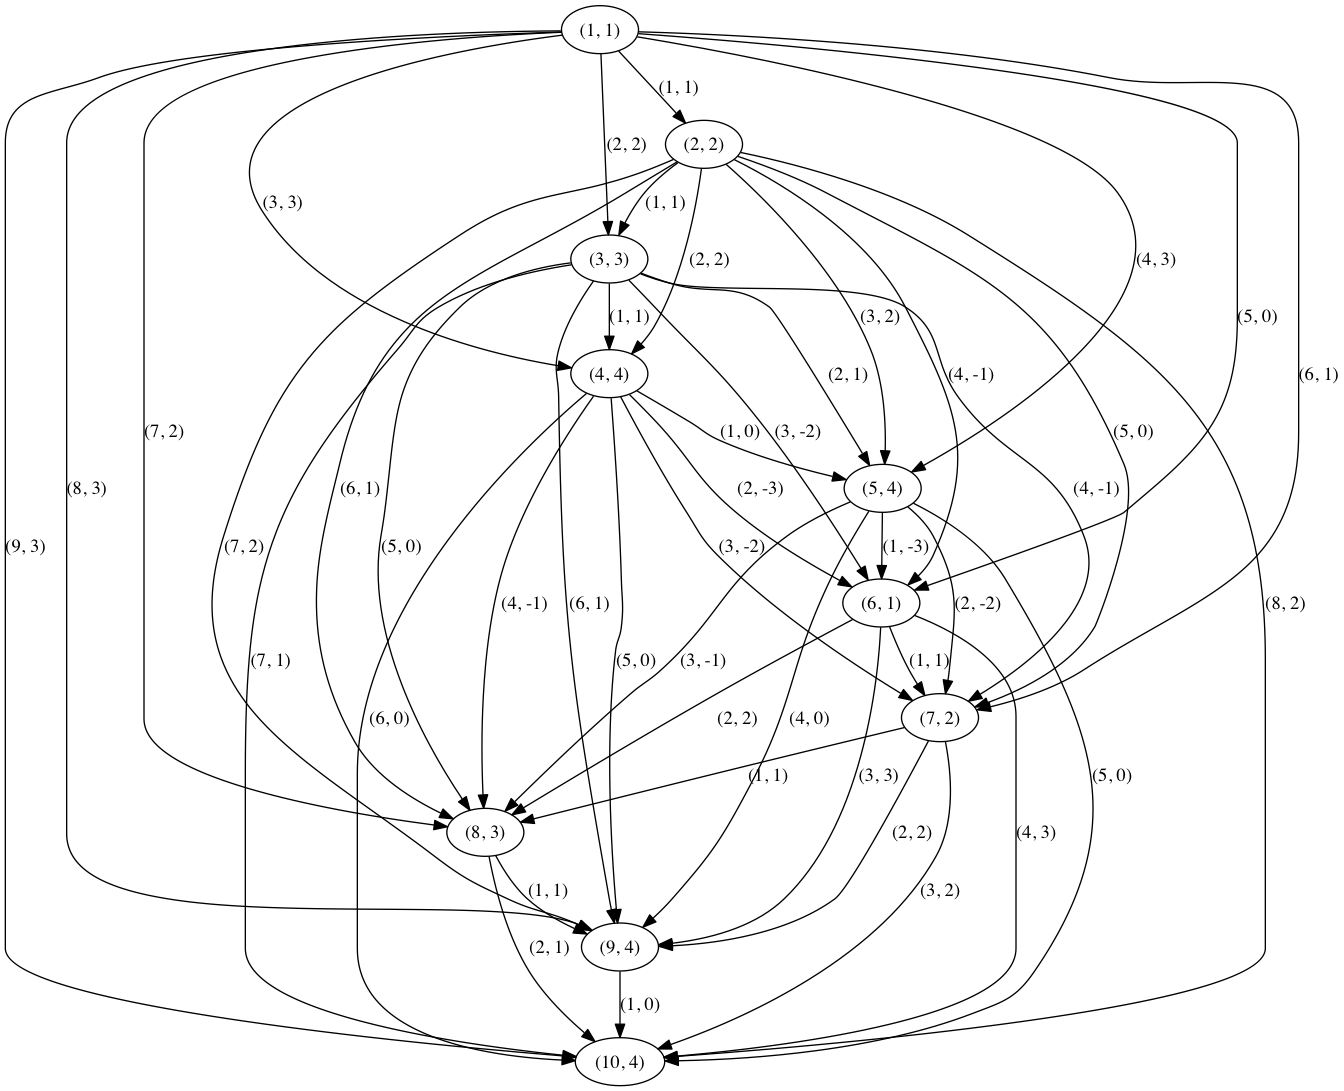
\includegraphics[width=\textwidth]{optimal_check}
  \label{fig:figure2}
  \caption{A digraph depicting all vector shifts from every point to every subsequent point in the dataset shown in figure 1. Nodes in this graph represent points in the dataset, and arcs represent the vector shifts from a point to another point. The arcs are labeled with the vector shift required to travel from the initial point to the ending point.}
\end{figure}
\FloatBarrier

We will now demonstrate an example occurrence of an instance of a TEC set that requires identifying a pattern other than the pattern instances discovered by computing the MVS set associated with the pattern. Consider the reconstruction of the dataset shown below with an annotated TEC consisting of three instances of a pattern:

\FloatBarrier
\begin{figure}[!htbp]
  \centering
  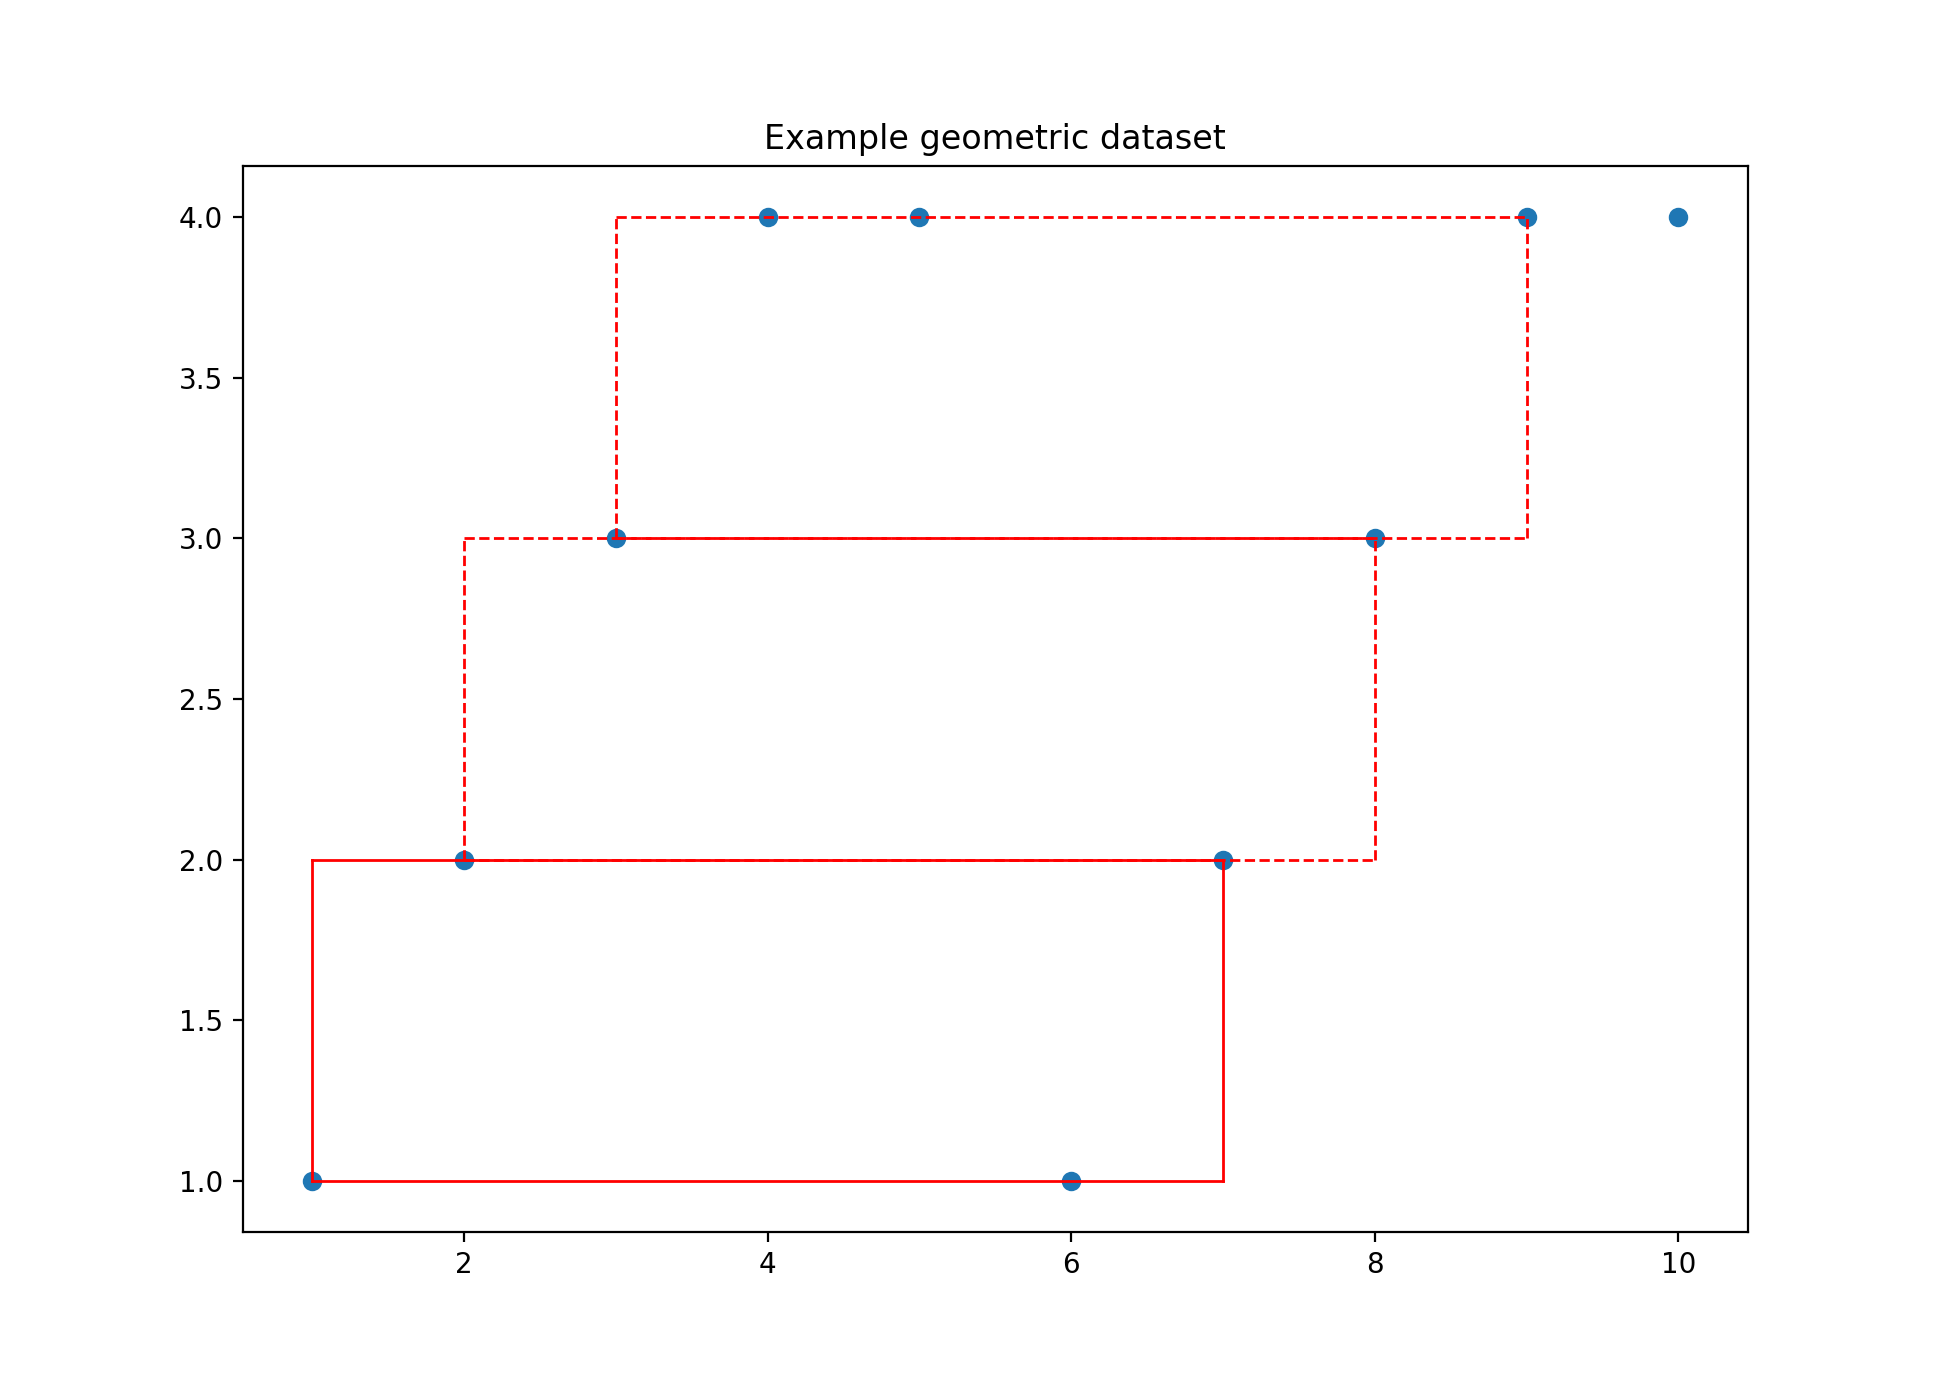
\includegraphics[width=.8\textwidth]{annotated_data_example}
  \label{fig:figure3}
  \caption{A TEC found in our example dataset. This TEC is defined by: $\left\{ P:\{(1, 1); (2, 2); (6, 1); (7, 2)\}; T: \{(0, 0); (1, 1); (2, 2)\} \right\}$}
\end{figure}
\FloatBarrier

For this instance if we reference figure 2 we see that the first instance of the pattern for this TEC (outline in solid red in figure 3) is found when computing the MVS set for the vector (2, 2). This also discovers the third instance of the pattern. However, computing the MVS does not discover the second instance of the pattern, because the actual vector shift from the second instance of the pattern to the third instance of the pattern is (1, 1) and the shift from the second instance of the pattern to the first instance is (1, -1). The (1, 1) vector pattern has a MVS associated with it that is greater in size than the MVS for (2, 2) and thus we do not discover the pattern from this computation. The (1, -1) vector shift does not exist for this dataset because of how we defined an ordering on the points in the dataset and the start point we chose for computing the vector shifts from any point to all subsequent points. Illuminating this fact shows why cubic time is required to find all possible instances of all MTPs to form TEC sets. If we were to consider every possible starting position and compute MVS sets based upon the vectors discovered from said starting position then we would uncover all MTPs and be able to create fully formed TEC sets. For instance, setting (2, 2) as the starting point and modulating all points around it to hold to the same ordering rules would reveal an MVS set that includes the second pattern instance shown in figure 3. Furthermore we cannot be guaranteed to recover all unique instances of every MTP found in the dataset without considering every starting point, as shifting the starting point will determine which MVS sets are computed by the corresponding vectors between the points in the dataset with their corresponding subsequent points. There are $n$ possible starting points and for each starting point we must compute the MVS sets from all possible vector shifts, an operation which has been shown to take $O(n^2)$ time. Performing an $O(n^2)$ time operation $n$ times means that the computation time to compute the TEC sets takes $O(n^3)$ time.

\section{The HashTEC Algorithm}
Now that we have established the inability to perform the original task of computing all TECs that exist in $D$ in quadratic time we will introduce a new algorithm we developed that is still applicable to generation. As discussed in the section above the aggregated arc sets can be computed in quadratic time, and performing this computation will guarantee that at-least two instances of all MTPs present in $D$ will be found. From this result we constructed the HashTEC algorithm, which is designed to discover all patterns present in a geometric dataset in quadratic time. In this section we will present the detailed algorithm behind HashTEC and analyze the algorithms runtime. We will then present comparative results between SIATEC and HashTEC on both synthetic datasets and real-world 2-dimensional music datasets. The report will then conclude with a discussion on potential use-cases of HashTEC for on-line constraint based generation.
	
The HashTEC algorithm is split into three sections. The first section takes $O(n^2)$ time to complete, and the following two take $O(k)$, where k is the input vector shift table computed in the first section. Given a dataset consisting of tuples representing points on a graph, we first compute a list of vector shifts corresponding to the difference in position between every pair of points on the graph. Since we don't need to re-compute point differences if they have already been compared once before, we can get away with using a list of size $\frac{(n^2)}{2}$. The algorithm for this section is laid out as follows: 
V is the list of vector shifts we wish to calculate. For every point v1 in D, where D is the given Dataset, and for every point v2 that has not yet been compared to v1:  compute v1 - v2 and store the result in list V along with the corresponding index of v1. Return V. We can see that the number of items k produced by this section is equivalent to k = $\frac{n(n-1)}{2}$, and this results in a total runtime of $O(n^2)$.

The second section of the algorithm takes in the list computed in the first section, and outputs a hash table where keys are computed vector shifts, and the corresponding value is a list containing all of the point indices that can be shifted by the amount in the key. This part of the algorithm works as follows: Let M be the hash table of vector shifts we wish to compute. For every vector shift v in the input list V, and every index i associated with that vector shift: if v exists in the table M, we append the index i to the end of the list corresponding to v, otherwise we create a new entry in M with key = v and value = list containing i. Return M. This section takes in k values in a list, and visits each item exactly once, resulting in a runtime of $O(k)$.

The last step in the algorithm is to create a hash table containing all of the MTPs we have found so far. To calculate this we take the difference between points found corresponding to a particular vector shift, and then hash the resulting shifts between those points as a key into the table. Since we are not interested in the occurrences of each pattern, just the pattern itself, we do not put a value in the table associated with each key. The algorithm computes as follows: For each vector shift and associated set of point P in table M, if the cardinality of P is larger than 1: initialize a Max Vector Shift list T containing the default vector shift of (0,0). Then for each point in the set P: compute the difference between P1 and P2, and append the result to the end of list T. After looping through P, insert the list T as a key into the table. Finally, return the set of keys in the MTP table. Like before, this section takes in k values in a list, and visits each item exactly once, resulting in a runtime of $O(k)$. The overall runtime of the algorithm is thus equal to $O(n^2)$ + $O(k)$ + $O(k)$, which results in a total overall runtime of $O(n^2)$.


\section{Algorithm Comparison Results}
Our results are meant to show the advantage of using the HashTEC algorithm in terms of time required to discover of all patterns present in a dataset. We first tested our algorithm on synthetic datasets designed to test the algorithms abilities to handle regular geometric data. In order to make our data as regular as possible we used randomly generated datasets. The figure below shows the comparative results for the two algorithms on 3 synthetic randomly generated datasets ranging from size of 10 data points to 500 data points. The figure shows that the runtime for SIATEC increase much faster than HashTEC as the size of the dataset increases.
\FloatBarrier
\begin{figure}[!htbp]
  \centering
  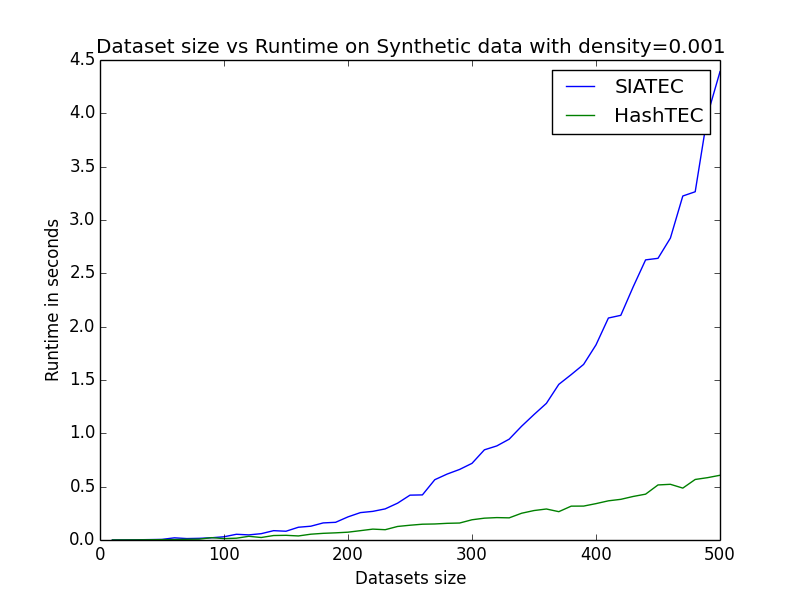
\includegraphics[width=.3\textwidth]{prelim_results_0}
  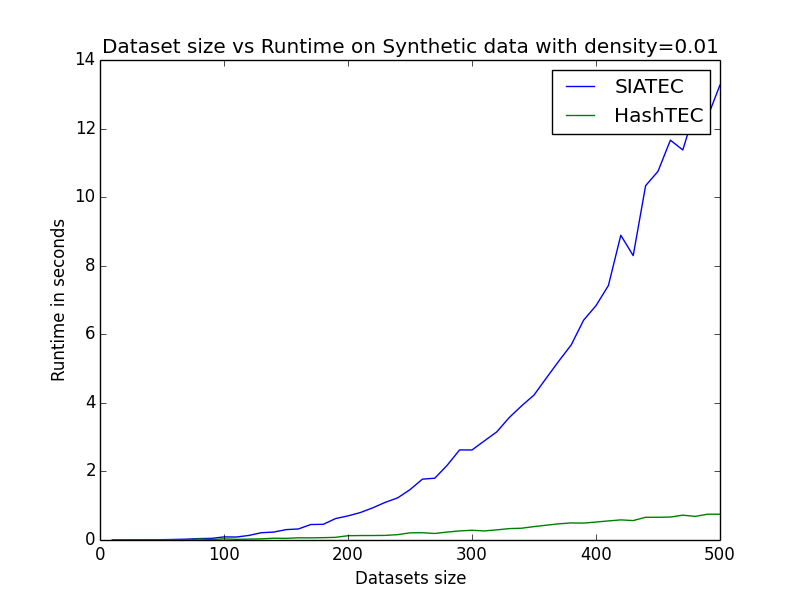
\includegraphics[width=.3\textwidth]{prelim_results_1}
  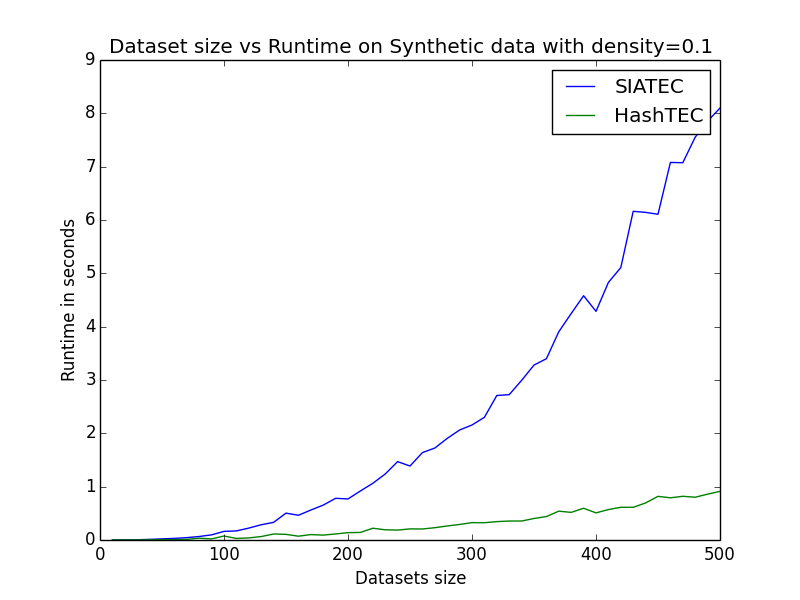
\includegraphics[width=.3\textwidth]{prelim_results_2}
  \label{fig:figure4}
  \caption{Preliminary results showing the differences in runtime of SIATEC and HashTEC on synthetic data, varying point density by 0.001, 0.01, and 0.1. Note how the y axis values differ between the graphs on the far left and the far right, compared to the relatively larger y axis values in the center graph.}
\end{figure}
\FloatBarrier

It is important to note for the three figures shown above that the difference between the three datasets analyzed was the density of the randomly generated points. We theorized that density for randomly generated points would affect the number of patterns present in the dataset. The figure below shows the number of unique patterns found in each of the datasets for both the SIATEC and HashTEC algorithms. We have included the results for each just as a visual confirmation that the number of patterns returned by both algorithms is indeed equivalent. Notice that the second dataset has considerably more patterns than the other two. Now look back to figure 4 and notice that the y-axis of the middle plot has values much higher than that of the other two plots. Although SIATEC has the same functional form for runtime on this plot as the other two, the actual runtime values are much higher due to many more patterns being present in the dataset. Recall that all three of these datasets have the same number of points. This implies that the time complexity of SIATEC is a function of the number of patterns found in the dataset. This is not the case for HashTEC, and the benefit of not increasing the runtime of an algorithm based upon the number of results independent of an increase in the size of the underlying dataset is another attractive feature of the HashTEC algorithm.

\FloatBarrier
\begin{figure}[!htbp]
  \centering
  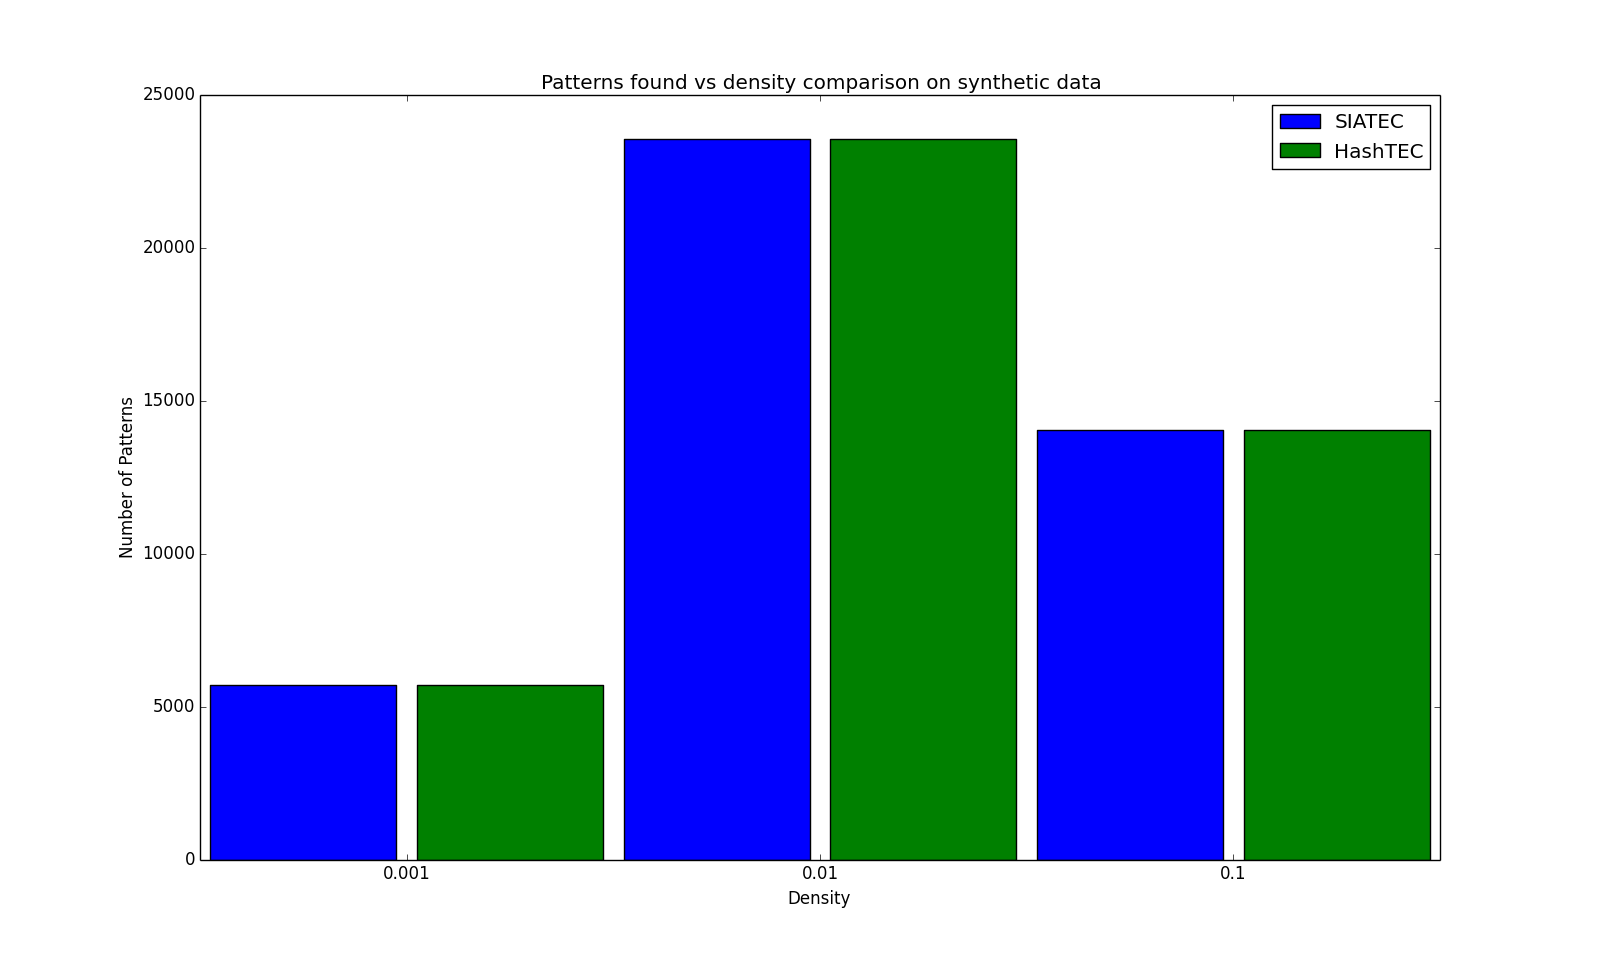
\includegraphics[width=.8\textwidth]{patterns_found_vs_density_synthetic_data}
  \label{fig:figure5}
  \caption{Chart comparing the differences in number of patterns found versus point density between SIATEC and HashTEC for synthetic data. Note how a density of 0.01 results in higher number of patterns found when compared to a density of 0.001 and 0.1}
\end{figure}
\FloatBarrier

After conducting experiments on synthetic data we desired to compare the performance of the two pattern finding algorithms on music data. For this test we compared the runtimes of the two algorithms on a collection of complete solos from a corpus of Charlie Parker music. The runtime results are shown below, on every solo HashTEC performs the computations required much faster than the SIATEC algorithm. This verifies that our results can be used for real-world data and applications.

\FloatBarrier
\begin{figure}[!htbp]
  \centering
  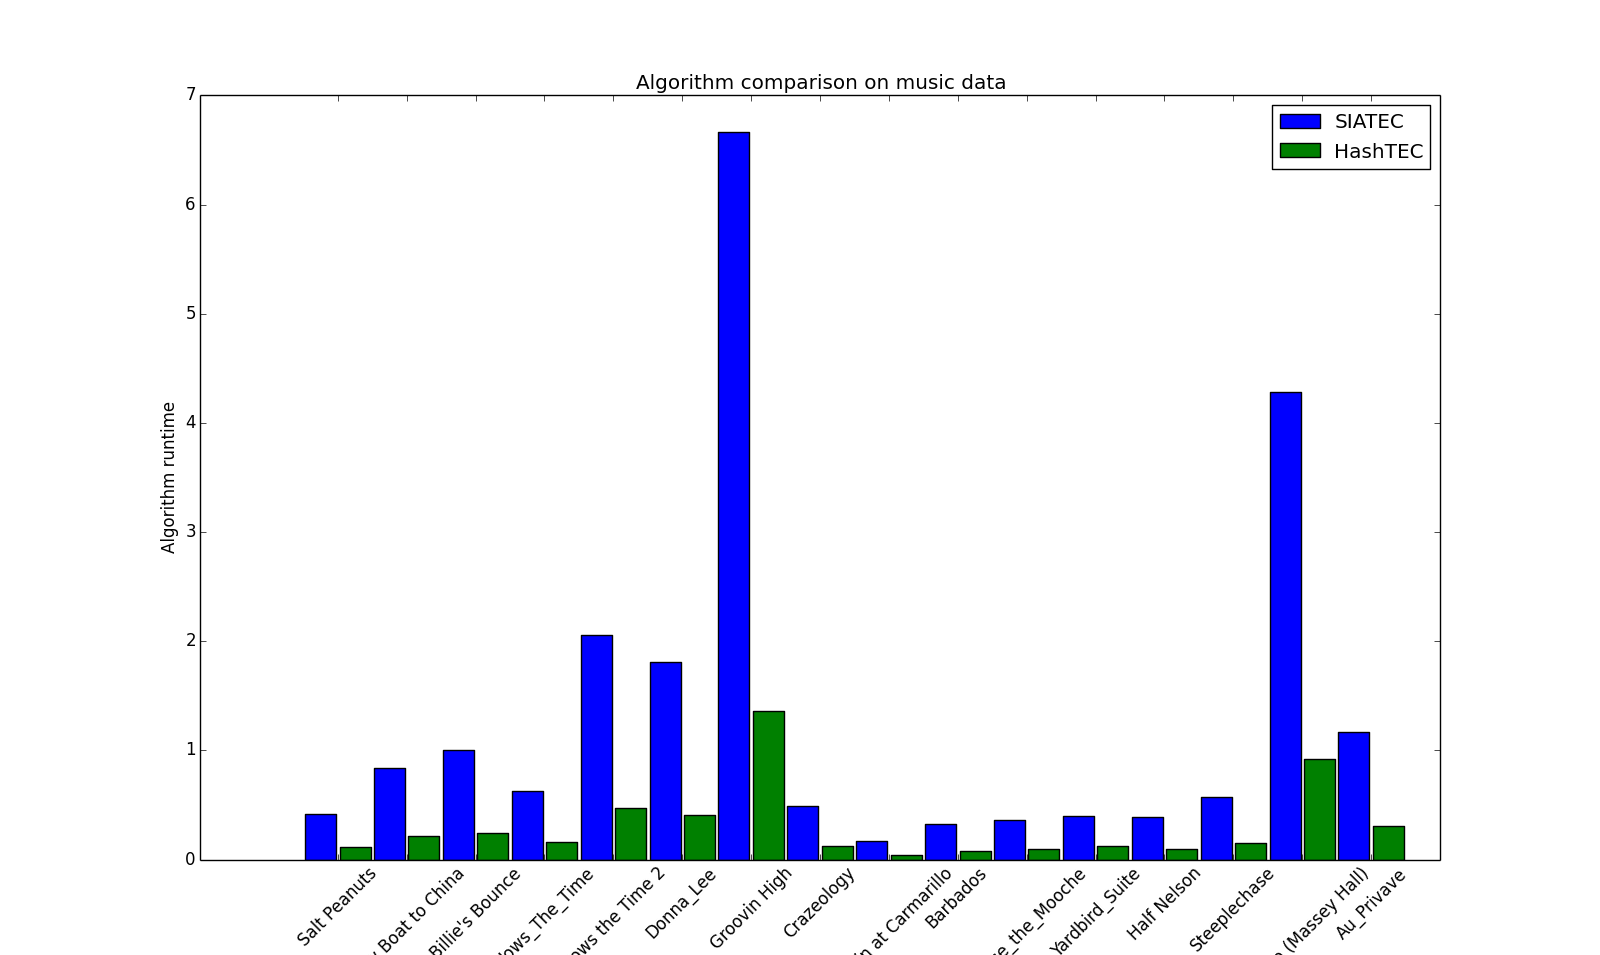
\includegraphics[width=.8\textwidth]{comp_algs_runtimes_on_music}
  \label{fig:figure6}
  \caption{Chart comparing runtime for each algorithm on different sets of music data.}
\end{figure}
\FloatBarrier

Similar to our synthetic data studies we also desired to consider the number of patterns found when considering the runtime of the two algorithms on the datasets. Below is a figure that shows the number of patterns found for each music piece that can be referenced when considering the disparity in runtimes between music pieces and between the two algorithms.

\FloatBarrier
\begin{figure}[!htbp]
  \centering
  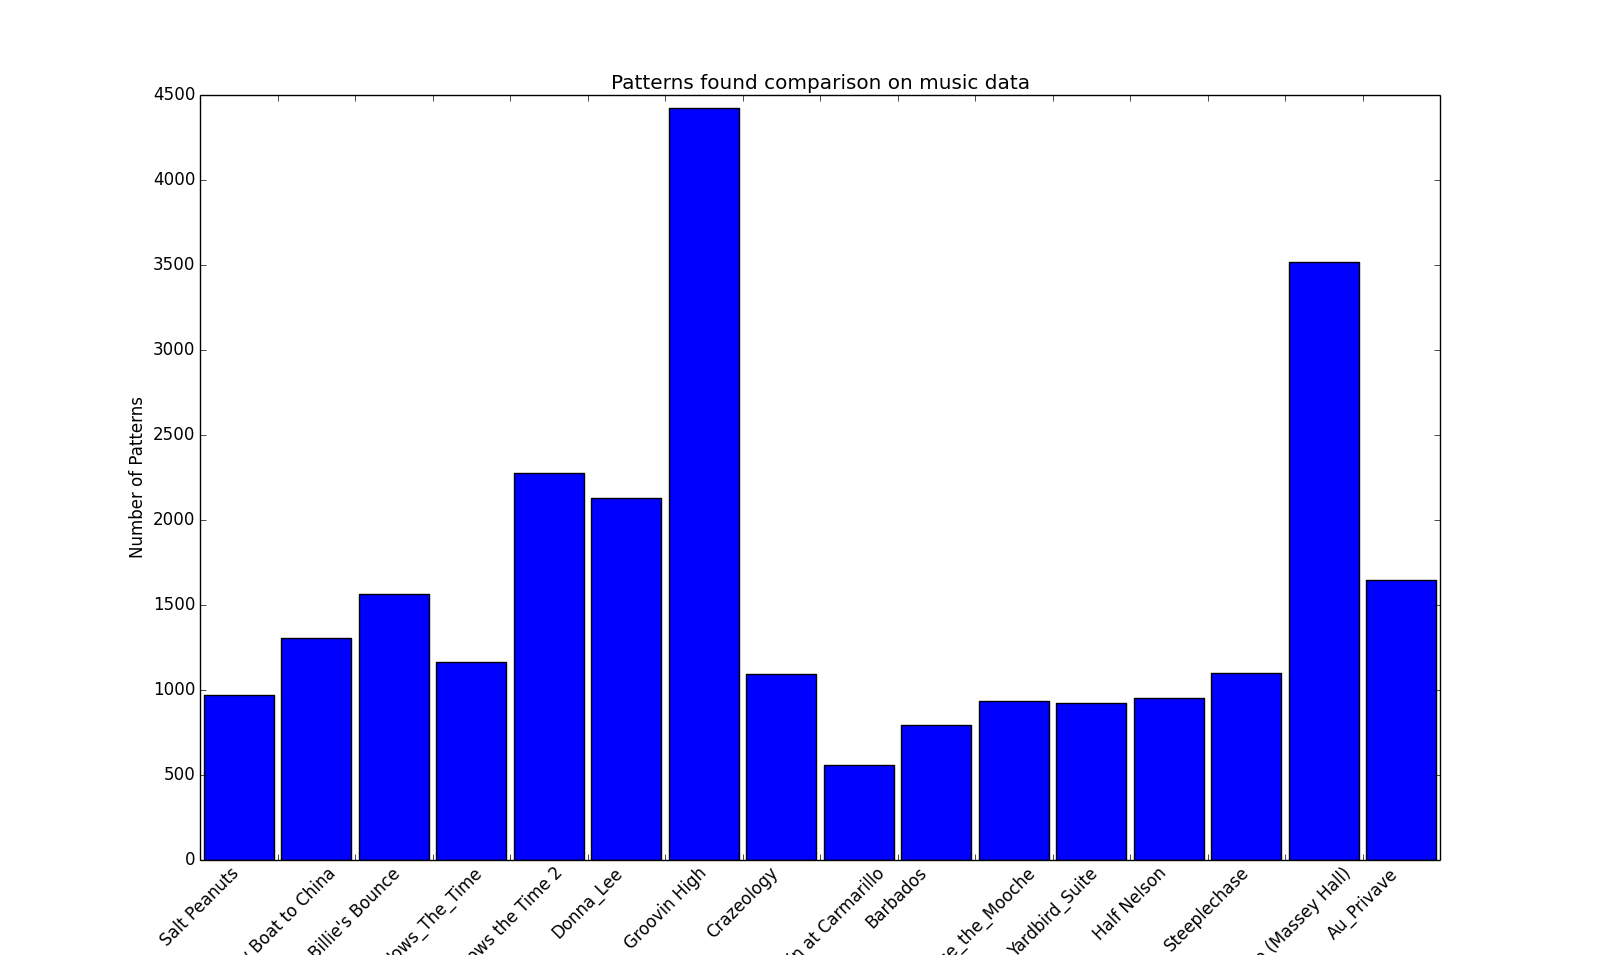
\includegraphics[width=.8\textwidth]{patterns_found_comp_music_data}
  \label{fig:figure7}
  \caption{Chart comparing the number of patterns found for each algorithm in each piece in the set of music data.}
\end{figure}
\FloatBarrier


\section{Discussion}
Both algorithms discussed in this report are concerned with finding geometric patterns in a k-dimensional dataset $D$. The key difference between SIATEC and HashTEC is that SIATEC is concerned with finding and grouping all instances of all patterns in $D$. This implies that SIATEC must solve the following problems: duplicate pattern problem, discovery of sub-maximal patterns for a given vector shift, and identifying only maximal TEC sets. These problems require SIATEC to increase its algorithmic runtime from $O(n^2)$ to $O(n^3)$, an increase which does not allow for fast on-line generation when ran over large amounts of input. In contrast the HashTEC algorithm, which only outputs the patterns present in $D$ and does not recover the number of instances or instance locations of each instance of each pattern, can compute in $O(n^2)$ time making on-line generation more feasible for larger input datasets.
\\
\\HashTEC is a preferable algorithm to SIATEC for discovering patterns that will be used for constraint-based generation if the following condition is met: the use case must not require the number of occurrences of pattern in $D$, nor the locations of occurrences of a pattern in $D$. This is an unfortunate restriction, but there are still generation schemes that can make use of this result. Consider a generation scheme that treats all patterns found in a training dataset as an unweighted bag. A generation scheme that randomly samples from this bag without a weighting on the number of occurrences for patterns in the bag can make use of the HashTEC algorithm to compute all patterns included in the bag for generation. In fact patterns used for generation can still be weighted based upon the pattern length and other use-case dependent definitions of pattern complexity. An example of this would be patterns based upon the number of components, the number of contour changes in one or more of the axes, or the number of points in a pattern that share a value for one or more axes. These simple examples show that the pattern-types still encode large amounts of information useful for constraint-based generation and therefore the HashTEC algorithm is definitely of interest to use-cases that involve on-line constraint-based generation of geometric data.

\begin{thebibliography}{9}
\bibitem{SIATEC_Paper}
Meredith, D., Lemström, K., \& Wiggins, G. A. (2002). \textit{Algorithms for discovering repeated patterns in multidimensional representations of polyphonic music.} Journal of New Music Research, 31(4), 321–345. https://doi.org/10.1076/jnmr.31.4.321.14162
\end{thebibliography}

\end{document}